%%%%%%%%%% *** The Title %%%%%%%%%%
\title[]{기압과 바람\\\small{제6장}}

\begin{frame}[plain] %title page
	\titlepage
\end{frame}


\section{기압과 바람}



\begin{frame}[t]{기압}
	\begin{tabular}{ll}
		\begin{minipage}[t]{0.45\textwidth}\scriptsize
			\begin{figure}[t]
				\includegraphics[trim=320 320 50 140, clip, page=189, width=\textwidth]{\bookfile}
			\end{figure}
		\end{minipage}	
		&
		\begin{minipage}[t]{0.45\textwidth} \scriptsize	
			바람은 기압의 수평방향 차이에 의한 결과
			기압은 공기의 무게에 의하여 받는 단위 면적당의 힘\\
			
			과거에는 milibar 단위를 사용했으나 최근에는 $\rm{~hPa}$ 단위를 사용 $\left(1 \rm{~mb} = 1 \rm{~hPa} = 100 {~N/m^2}\right)$\\
			
			\questionset {해수면에서의 대기압을 $\rm{hPa}$ 단위로 계산하시오.}
			\solutionset{
			 $${\displaystyle {
			 		\begin{aligned}
			 			1 \textrm{~기압} &= 1 \rm{~atm} = 76 \rm{~cmHg} \\
			 			P &= \rho g h \\
			 			&= 13.595 \rm{~g/cm^3} \times 9.80665 \rm{~m/s^2} \times 76 \rm{~cm}  \\
						&= 13595 \rm{~kg/m^3} \times 9.80665 \rm{~m/s^2} \times 0.76 \rm{~m} \\
						&= 101324.27 \rm{~kg/m^3 s^2} \\
						&= 1013.2427 \rm{~kg~m~s^2/m^2} \\
						&= 1013.2427 \rm{~hPa}
 			 		\end{aligned}
 		 		}	}$$}
		\end{minipage}
	\end{tabular}
\end{frame}






\begin{frame}[t]{기압의 측정}
	\begin{tabular}{ll}
		\begin{minipage}[t]{0.475\textwidth}\scriptsize
			\begin{figure}[t]
				\includegraphics[trim=50 385 320 50, clip, page=190, width=0.85\textwidth]{\bookfile}
			\end{figure}
			
		\end{minipage}	
		&
		\begin{minipage}[t]{0.475\textwidth} \scriptsize	
			\begin{figure}[t]
				\includegraphics[trim=50 30 320 410, clip, page=190, width=0.8\textwidth]{\bookfile}
			\end{figure}	
				수은기압계: 토리첼리가 발명한 것으로 수은을 사용
		\end{minipage}
	\end{tabular}
\end{frame}



\begin{frame}[t]{기압의 측정}
	\begin{tabular}{ll}
		\begin{minipage}[t]{0.4\textwidth}\scriptsize
			\begin{figure}[t]
				\includegraphics[trim=350 30 50 410, clip, page=190, width=0.8\textwidth]{\bookfile}
			\end{figure}
			아네로이드 기압계 : 진공의 금속관을 사용하여 기압의 증감에 따라 수축하거나 팽창하면서 진공관의 형태가 바뀌게 됨. 
		\end{minipage}	
		&
		\begin{minipage}[t]{0.55\textwidth} \scriptsize	
			\begin{figure}[t]
				\includegraphics[trim=30 520 350 60, clip, page=191, width=0.9\textwidth]{\bookfile}
			\end{figure}
			아네로이드 기압 기록계: 연속적으로 기압 값을 기록함.
		\end{minipage}
	\end{tabular}
\end{frame}







\begin{frame}[t]{기압의 해면 경정}
	\begin{tabular}{ll}
		\begin{minipage}[t]{0.6\textwidth}\scriptsize
			\begin{figure}[t]
				\includegraphics[trim=40 50 270 540, clip, page=191, width=\textwidth]{\bookfile}
			\end{figure}
		\end{minipage}	
		&
		\begin{minipage}[t]{0.35\textwidth} \scriptsize	
			고도에 따른 기압의 변화를 보정하기 위해 해수면에서의 값으로 관측값을 환산해야 함.\\
			일반적으로 해수면 근처에서는 $10 \rm{~m}$ 상승시 $1 \rm{~hPa}$ 감소.
		\end{minipage}
	\end{tabular}
\end{frame}





\begin{frame}[t]{지상 일기도}
	\begin{tabular}{ll}
		\begin{minipage}[t]{0.65\textwidth}\scriptsize
			\begin{figure}[t]
				\includegraphics[trim=50 450 230 60, clip, page=192, width=\textwidth]{\bookfile}
			\end{figure}
			
		\end{minipage}	
		&
		\begin{minipage}[t]{0.3\textwidth} \scriptsize	
			
			지상 일기도에는 해면 기압이 같은 지점을 연결한 등압선을 표시함.\\
			
			붉은색 화살표는 바람을 나타냄.\\
	
			\questionset{고기압, 저기압의 수평적 크기는 얼마나 되는가?}
			\solutionset{대개 $1000 \sim 2000 \rm{~km}$ 정도의 크기를 갖는다. }
		\end{minipage}
	\end{tabular}
\end{frame}


\begin{frame}[t]{상층 일기도}
	\begin{tabular}{ll}
		\begin{minipage}[t]{0.6\textwidth}\scriptsize
			\begin{figure}[t]
				\includegraphics[trim=270 30 30 430, clip, page=192, width=\textwidth]{\bookfile}
			\end{figure}
			
		\end{minipage}	
		&
		\begin{minipage}[t]{0.35\textwidth} \scriptsize	
			
			상층 일기도는 등압면에 대한 등고선으로 나타냄\\

			기압이 높은 곳은 기압마루(ridge), 기압이 낮은 곳은 기압골(trough)\\
			
			붉은색 화살표는 바람을 나타냄.\\
		
			\questionset{기상청에서 제공하는 상층 일기도의 종류와 대략적인 고도는?}
			\solutionset{$925 \rm{~hPa} : 800\rm{~m}$,\\
				$850 \rm{~hPa} : 1,500\rm{~m}$,\\
				$700 \rm{~hPa} : 3,000\rm{~m}$,\\
				$500 \rm{~hPa} : 5,600\rm{~m}$,\\
				$300 \rm{~hPa} : 9,800\rm{~m}$,\\
				$200 \rm{~hPa} : 12,500\rm{~m}$,\\
				$100 \rm{~hPa} : 16,800\rm{~m}$}
		\end{minipage}
	\end{tabular}
\end{frame}







\section{기압은 왜 변하는가}



\begin{frame}[t]{고도에 따른 기압의 변화}
	\begin{tabular}{ll}
		\begin{minipage}[t]{0.4\textwidth}\scriptsize
			\begin{figure}[t]
				\includegraphics[trim=50 470 440 50, clip, page=194, width=0.70\textwidth]{\bookfile}
			\end{figure}
		
				고도가 높아질수록 위에서 누르는 공기의 무게가 줄어들기 때문에 기압이 감소한다.
		\end{minipage}	
		&
		\begin{minipage}[t]{0.55\textwidth} \scriptsize	
			\begin{figure}[t]
				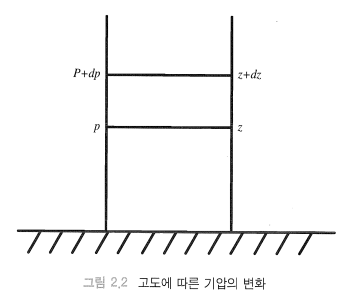
\includegraphics[width=0.70\textwidth]{./images/rgh}
			\end{figure}
			기압의 감소율은 로그 스케일로 지상에 가까울수록 감소율이 크고, 상공에서는 작다.\\
			$${\displaystyle	{
				-\nu \frac{dp}{dz} = g \quad 				\frac{dp}{dz} = -\rho g
			}}$$
		\end{minipage}
	\end{tabular}
\end{frame}


\begin{frame}[t]{기온에 따른 기압의 변화}
	\begin{tabular}{ll}
		\begin{minipage}[t]{0.50\textwidth}\scriptsize
			\begin{figure}[t]
				\includegraphics[trim=350 135 50 385, clip, page=194, width=\textwidth]{\bookfile}
			\end{figure}
			
		\end{minipage}	
		&
		\begin{minipage}[t]{0.45\textwidth} \scriptsize	
				기온이 높을수록 분자운동이 더 활발하여 입자간 거리가 멀고 밀도가 작다.\\
				밀도가 증가하면 지표면에 미치는 기압이 커지게 된다.\\
				다른 조건이 모두 같다면, 차가운 공기는 지상의 고기압, 따뜻한 공기는 지상의 저기압이 된다.\\
				찬 공기(밀도가 큰 공기)의 경우 따뜻한 공기(밀도가 작은 공기)에 비하여 고도에 따른 기압 감소가 크다.\\
				높은 고도에서는 따뜻한 지역이 찬 지역 보다 더 높은 기압을 갖게 된다.
		\end{minipage}
	\end{tabular}
\end{frame}





\begin{frame}[t]{기압의 변화}
	\begin{tabular}{ll}
		\begin{minipage}[t]{0.475\textwidth}\scriptsize
			
		\end{minipage}	
		&
		\begin{minipage}[t]{0.475\textwidth} \scriptsize	
			\questionset{기압이 변하는 요인 네 가지를 설명하시오.}
			\solutionset{1)고도: 고도가 높아질수록 위에서 누르는 공기의 무게가 줄어들기 때문에 기압이 감소\\
				기압의 감소율은 로그 스케일로 지상에 가까울수록 감소율이 크고, 상공에서는 작다.\\
			2)기온: 기온이 높을수록 분자운동이 더 활발하여 입자간 거리가 멀고 밀도가 작음. 이에 따라 기압도 작아짐
			3)수증기량: 수증기량이 많을수록 공기의 밀도가 낮아져 기압은 감소\\
			일반적으로 지상에서 차고 건조한 공기는 습하고 따뜻한 공기보다 지상에 더 높은 기압 발생시킴.\\
			4) 상층의 공기 흐름: 상층 수렴은 지상 기압 상승을, 상층 발산은 지상 기압 하강을 유도}
		\end{minipage}
	\end{tabular}
\end{frame}




\begin{frame}[t]{기압의 변화}
	\begin{tabular}{ll}
		\begin{minipage}[t]{0.9\textwidth}\scriptsize
			\begin{figure}[t]
				\includegraphics[trim=220 485 180 100, clip, page=195, width=0.49\textwidth]{\bookfile}
				\includegraphics[trim=220 280 180 310, clip, page=195, width=0.49\textwidth]{\bookfile}
			\end{figure}			
		\end{minipage}	
		&
		\begin{minipage}[t]{0.05\textwidth} \scriptsize	
		\end{minipage}
	\end{tabular}

		\questionset{산악 지형을 비행하는 경우 위험한 결과를 초래할 수 있는 이유는?}
		\solutionset{비행 고도계는 기압을 고도로 바꾸어주는 아네로이드 기압계로 구성되어 있다. 
			항상 변화하는 기압과 기온으로 인해 비행기 내부 기록된 기압이 실제와 달라진다.\\
			표준대기 보다 따뜻한 곳은 고도계의 고도보다 더 높은 고도 비행,\\
			표준대기 보다 차가운 곳은 고도계의 고도보다 더 낮은 고도 비행}
\end{frame}






\section{바람에 영향을 미치는 요소}



\begin{frame}[t]{기압경도력(PGF, Pressure Gradient Force)}
	\begin{tabular}{ll}
		\begin{minipage}[t]{0.9\textwidth}\scriptsize
			\begin{figure}[t]
				\includegraphics[trim=40 525 350 50, clip, page=197, width=0.32\textwidth]{\bookfile}
				\includegraphics[trim=40 320 350 267, clip, page=197, width=0.32\textwidth]{\bookfile}
				\includegraphics[trim=40 70 350 475, clip, page=197, width=0.32\textwidth]{\bookfile}
			\end{figure}
			
		\end{minipage}	
		&
		\begin{minipage}[t]{0.05\textwidth} \scriptsize	
			
		\end{minipage}
	\end{tabular}
	
			\questionset{온도 차이가 수평 기압 경도와 이에 따른 바람을 생성하는 과정을 ‘해풍’의 예로 설명하시오.}
			\solutionset{일출 후 육지는 기온 상승, 바다는 큰 변화 없음. 이에 따라 육지쪽 공기가 데워져서 팽창하고 밀도 감소. \\
				특정 고도 위에서는 따뜻한 쪽의 공기가 차가운 쪽의 공기보다 기압이 높아짐. 이에 따라 상층에서는 육지에서 바다로 바람이 분다.\\
				상층 바람으로 바다쪽에 공기가 많이 쌓이게 되어 지상 기압 상승하며, 반대로 육지쪽은 지상 기압 감소. 지상 부근에서는 바다에서 육지쪽으로 바람이 불게 됨. 완전한 순환을 위해 연직방향 운동도 존재함. }

\end{frame}



\begin{frame}[t]{기압경도력(PGF)}
	\begin{tabular}{ll}
		\begin{minipage}[t]{0.45\textwidth}\scriptsize
			\begin{figure}[t]
				\includegraphics[trim=350 40 30 420, clip, page=196, width=\textwidth]{\bookfile}
			\end{figure}
		\end{minipage}	
		&
		\begin{minipage}[t]{0.5\textwidth} \scriptsize	
				\begin{figure}[t]
					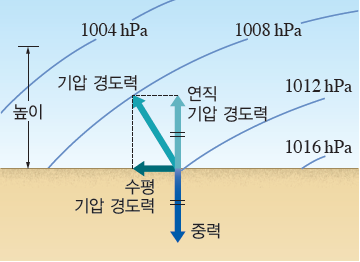
\includegraphics[width=0.7\textwidth]{./images/PGF.png}
				\end{figure}
			등압선의 간격이 좁을수록, 기압경도력이 크고, 바람이 강하다.\\
			기압경도력은 등압선에 직각 방향으로 기압이 높은 곳에서 낮은 곳으로 작용함\\
			연직 기압경도력은 중력과 상쇄되므로, 바람을 일으키는 근본적인 힘은 수평 기압 경도력임. \\
			기압의 차이에 의해 작용하는 힘으로 주로 수평 방향의 바람을 일으키는 근원적인 힘이다.
		\end{minipage}
	\end{tabular}
\end{frame}




\begin{frame}[t]{기압경도력(PGF)}
	\begin{tabular}{ll}
		\begin{minipage}[t]{0.5\textwidth}\scriptsize
			\begin{figure}[t]
				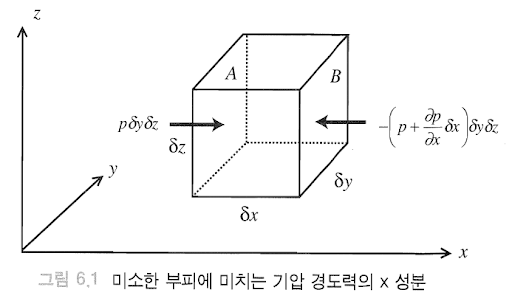
\includegraphics[width=\textwidth]{./images/PGF1}
			\end{figure}
		\end{minipage}	
		&
		\begin{minipage}[t]{0.45\textwidth} \scriptsize	
			압력은 단위 면적에 수직으로 작용하는 힘으로 정의되므로 정육면체 공기덩이에 작용하는 힘은 기압과 힘을 받는 면의 넓이의 곱으로 표현할 수 있다. \\
			
			단위 질량 당 기압경도력을 $x$, $y$,  $z$ 각 성분별로 단위 벡터 $\boldsymbol{\hat{i}}$,  $\boldsymbol{\hat{j}}$, $\boldsymbol{\hat{k}}$	로 기압경도력을 표현하면 
			$${\displaystyle	{
					\frac{F_{PGF}}{m}=-\frac{1}{\rho} \nabla p
			}	}$$
			
			$${\displaystyle	{
					\nabla=\frac{\partial}{\partial x} \boldsymbol{\hat i}+\frac{\partial}{\partial y} \boldsymbol{\hat j}+\frac{\partial}{\partial z} \boldsymbol{\hat k}
			}	}$$		
		\end{minipage}
	\end{tabular}
\end{frame}











\begin{frame}[t]{지상일기도에 표출된 등압선}
	\begin{tabular}{ll}
		\begin{minipage}[t]{0.9\textwidth}\scriptsize
			\begin{figure}[t]
				\includegraphics[trim=50 450 140 50, clip, page=198, width=0.85\textwidth]{\bookfile}
			\end{figure}
			
		\end{minipage}	
		&
		\begin{minipage}[t]{0.05\textwidth} \scriptsize	
			
		\end{minipage}
	\end{tabular}
	\scriptsize 
	지상 일기도에서 등압선은 대개 완만한 곡선으로 나타남.\\
	풍속의 단위로 노트($\rm{kn}$)를 많이 사용함. $1 \rm{~kn}$는 1 시간에 1 해리($1852 \rm{~m}$) 를 달리는 속도 ($1 \rm{~kn} = 0.51 \rm{~m/s}$)
\end{frame}




\begin{frame}[t]{전향력(Coriolis force)}
	\begin{tabular}{ll}
		\begin{minipage}[t]{0.9\textwidth}\scriptsize
			\begin{figure}[t]
				\includegraphics[trim=50 30 165 510, clip, page=198, width=0.8\textwidth]{\bookfile}
			\end{figure}
			
		\end{minipage}	
		&
		\begin{minipage}[t]{0.05\textwidth} \scriptsize	
			
		\end{minipage}
	\end{tabular}                  
	\scriptsize 
	코리올리 힘 자체는 바람을 발생시키지 못하고, 대신 바람의 방향을 변화시킨다.\\
	지구의 자전 때문에 북반구에서는 진행방향의 오른쪽 90도 방향으로 작용한다.\\
	지구상에 서있는 관측자가 로켓을 관찰하면 목표지점의 서편에 도착하는 것을 보게 된다.
\end{frame}



\begin{frame}[t]{전향력}
	\begin{tabular}{ll}                
		\begin{minipage}[t]{0.5\textwidth}\scriptsize
			\begin{figure}[t]
				\includegraphics[trim=50 430 250 50, clip, page=199, width=\textwidth]{\bookfile}
			\end{figure}
			
		\end{minipage}	
		&
		\begin{minipage}[t]{0.45\textwidth} \scriptsize	
			단위 질량당 작용하는 전향력은	
			$${\displaystyle	{
				\frac{F_{Col}}{m} = 2 v \Omega \sin \varphi  =fv
			}	}$$
			여기에서 $f = 2 \Omega \sin \varphi$는 코리올리 인자 이다.\\
			
			고위도일수록 전향력은 강하게 작용하며, 적도에서는 작용하지 않는다.			
		\end{minipage}
	\end{tabular}
\end{frame}



\begin{frame}[t]{전향력}
	\begin{tabular}{ll}
		\begin{minipage}[t]{0.5\textwidth}\scriptsize
			\begin{figure}[t]
				\includegraphics[trim=50 390 320 50, clip, page=200, width=\textwidth]{\bookfile}
			\end{figure}
			
		\end{minipage}	
		&
		\begin{minipage}[t]{0.45\textwidth} \scriptsize	
			남반구에서는 전향력의 방향이 진행방향의 왼쪽 방향이 된다.
		\end{minipage}
	\end{tabular}
\end{frame}


                                

\begin{frame}[t]{마찰력}
	\begin{tabular}{ll}
		\begin{minipage}[t]{0.45\textwidth}\scriptsize
			\begin{figure}[t]
				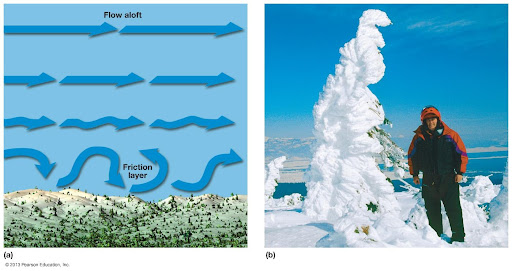
\includegraphics[trim=0 10 250 0, clip, width=\textwidth]{./images/friction}
			\end{figure}
			                                 
		\end{minipage}	       
			&
		\begin{minipage}[t]{0.5\textwidth} \scriptsize	
		
			마찰력이 존재하기 때문에 바람이 무한히 강하게 발달하지 않는다. \\ 
			지표 근처에서는 매우 중요하지만, 고도가 높아지면 무시 가능 \\
			경계층(약 고도 1.5km)에서만 중요
			
		\end{minipage}
	\end{tabular}
\end{frame}














\section{상층과 지상의 바람}




\begin{frame}[t]{상층 일기도}
	\begin{tabular}{ll}
		\begin{minipage}[t]{0.9\textwidth}\scriptsize
			\begin{figure}[t]
				\includegraphics[trim=50 370 50 50, clip, page=201, width=0.8\textwidth]{\bookfile}
			\end{figure}
			

		\end{minipage}	
		&
		\begin{minipage}[t]{0.55\textwidth} \scriptsize	
			
		\end{minipage}
	\end{tabular}

	\scriptsize 수 $\rm{km}$ 상층에서는 마찰력은 무시할 수 있다. 
\end{frame}
                    



                                       


\begin{frame}[t]{지균풍(Geostrophic wind)}
	\begin{tabular}{ll}
		\begin{minipage}[t]{0.4\textwidth}\scriptsize
			\begin{figure}[t]
				\includegraphics[trim=250 40 65 510, clip, page=201, width=\textwidth]{\bookfile}
			\end{figure}
			                                                 
		\end{minipage}	
		&
		\begin{minipage}[t]{0.55\textwidth} \scriptsize	
		상층에서 등압선이 직선일 때 구심력(원심력)이 작용하지 않는 경우에 기압경도력과 전향력이 균형을 이루어 등압선에 나란하게 바람이 분다.\\
		기압경도력에 의해 고기압⇒저기압 방향으로 공기가 움직이기 시작하면 북반구에서는 전향 력의 작용으로 공기의 운동방향이 오른쪽으로 휘어짐\\		
		기압경도력이 계속 작용하므로 공기의 속도는 더욱 빨라지며, 이에 따라 전향력도 더욱 커져서 공기의 운동방향이 더욱 오른쪽으로 휘어짐\\
		결국, 기압경도력과 전향력이 균형을 이루어 등압선과 나란한 바람(지균풍)이 불게 됨.\\
		Buys Ballot’s Law(보이스 발로트의 법칙)  : 북반구에서 바람을 등지고 있는 경우 왼쪽에 저기압이, 오른쪽에 고기압이 있음
		
		\end{minipage}
	\end{tabular}      
\end{frame}


                                       


\begin{frame}[t]{지균풍(Geostrophic wind)}
	\begin{tabular}{ll}
		\begin{minipage}[t]{0.4\textwidth}\scriptsize
			\begin{figure}[t]
				\includegraphics[trim=250 40 65 510, clip, page=201, width=\textwidth]{\bookfile}
			\end{figure}
			
		\end{minipage}	
		&
		\begin{minipage}[t]{0.55\textwidth}\scriptsize
			지균풍의 풍속 ($V_g$)는 다음과 같이 구할 수 있다.
				$${\displaystyle 	{
					\begin{aligned}
						f V_{g}&=-\frac{1}{\rho} \frac{\partial p}{\partial n} \quad
						V_{g}=-\frac{1}{f \rho} \frac{\partial p}{\partial n}\\
						f &= 2 \Omega \sin \varphi\\
						\Omega&=\frac{2 \pi}{23 \rm{^h} ~56 \rm{^m}}=7.29 \times 10^{-5} \rm{s^{-1}}
					\end{aligned}	
					}}$$
			 지균풍의 속력은 위도가 낮을수록, 등압선의 간격이 좁을수록 (기압경도력이 클수록) 빠름.
			
			\questionset{북반구 $30\rm{^\circ}$지역에서 $4 \rm{~hPa}$ 차이로 그린 등압선 간격이 $400\rm{~km}$이다. 공기의 밀도가 $1\rm{~g~m^{-3}}$ 일 때, 지균풍의 풍속을 구하시오.}
			\solutionset{$13.71 \rm{~m/s}$}
			
		\end{minipage}
	\end{tabular}
\end{frame}


\begin{frame}[t]{경도풍(Gradient wind)}
	\begin{tabular}{ll}
		\begin{minipage}[t]{0.55\textwidth}\scriptsize
			\begin{figure}[t]
				\includegraphics[trim=50 35 140 520, clip, page=202, width=\textwidth]{\bookfile}
			\end{figure}
		\end{minipage}	
		&
		\begin{minipage}[t]{0.4\textwidth} \scriptsize	
			상층에서 곡선의 등압선을 따라 일정한 속력으로 부는 바람으로, 기압경도력과 전향력의 차이가 구심력으로 작용한다.\\
			고기압성 경도풍의 경우
			$${\displaystyle	{
					\begin{aligned}
						-\frac{1}{\rho} \frac{\partial p}{\partial n}-f v&=\frac{v^{2}}{r}\\					
						f v&= -\frac{1}{\rho} \frac{\partial p}{\partial n} - \frac{v^{2}}{r}
					\end{aligned}
			}}	$$                       
			저기압성 경도풍의 경우
				$${\displaystyle	{
					\begin{aligned}
						f v+ \frac{1}{\rho} \frac{\partial p}{\partial n} &= \frac{v^{2}}{r}\\
						f v&= -\frac{1}{\rho} \frac{\partial p}{\partial n} + \frac{v^{2}}{r}					
					\end{aligned}
			}}	$$
		\end{minipage}
	\end{tabular}
\end{frame}





\begin{frame}[t]{경도풍(Gradient wind)}
	\begin{tabular}{ll}
		\begin{minipage}[t]{0.55\textwidth}\scriptsize
			\begin{figure}[t]
				\includegraphics[trim=50 35 140 510, clip, page=202, width=\textwidth]{\bookfile}
			\end{figure}
		\end{minipage}	
		&
		\begin{minipage}[t]{0.4\textwidth} \scriptsize	
			\questionset{저기압성 경도풍과 고기압성 경도풍의 풍속 및 지균풍의 풍속을 비교하고, 차이가 발생하는 이유는 무엇인지 경도풍의 힘의 균형을 이용하여 설명해 보자.}
			\solutionset{전향력은 풍속과 비례한다. 만약 등압선의 간격이 같다고 가정할 때, 고기압성 경도풍은 전향력의 크기가 기압경도력에 원심력 만큼 더한 것과 같고, 지균풍은 전향력의 크기가 기압경도력과 같으며, 저기압성 경도풍의 경우 전향력의 크기가 기압경도력에서 원심력 만큼 뺀 것과 같다. }
		\end{minipage}                                                    
	\end{tabular}
\end{frame}





\begin{frame}[t]{지상풍}
	\begin{tabular}{ll}
		\begin{minipage}[t]{0.6\textwidth}\scriptsize
			\begin{figure}[t]
				\includegraphics[trim=50 450 50 50, clip, page=204, width=\textwidth]{\bookfile}
			\end{figure}
		\end{minipage}	
		&
		\begin{minipage}[t]{0.35\textwidth} \scriptsize	
			지표에서 높이 약 $1\rm{~km}$까지는 마찰력이 작용하여 풍속이 느려지고 전향력도 줄어든다.\\
			이에 따라 전향력이 기압 경도력과 평형을 이루지 못하기 때문에 바람은 등압선을 가로질러 고기압에서 저기압으로 불게 됨.\\
			지표 부근에서 기압경도력, 전향력, 마찰력이 균형을 이루어 부는 바람을 지상풍이라고 함.
		\end{minipage}
	\end{tabular}
\end{frame}



\begin{frame}[t]{지상풍}
	\begin{tabular}{ll}
		\begin{minipage}[t]{0.4\textwidth}\scriptsize
			\begin{figure}[t]
				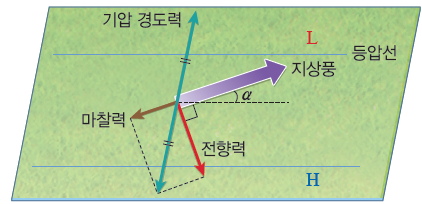
\includegraphics[width=\textwidth]{./images/SW2}
			\end{figure}

			등압선과 이루는 각(경각)을 $\alpha$ 라고 하면\\
				$${\displaystyle	{
						\begin{aligned}
							&\textrm{기압경도력} + \textrm{마찰력} + \textrm{전향력} = 0\\
							&\textrm{전향력} = \textrm{기압경도력} \times  \cos \alpha \\
							&\textrm{마찰력} = \textrm{기압경도력} \times  \sin \alpha
						\end{aligned}
				}}	$$

		\end{minipage}	
		&
		\begin{minipage}[t]{0.55\textwidth} \scriptsize	
			\begin{figure}[t]
				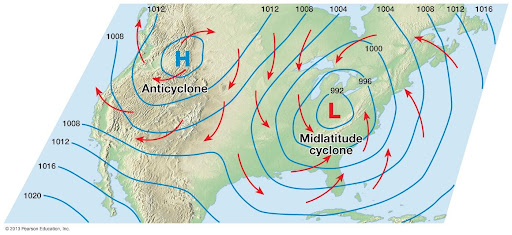
\includegraphics[width=\textwidth]{./images/surface_HL}
			\end{figure}

			마찰이 클수록 마찰을 극복하기 위해 $\alpha$가 크게 되어 등압선을 가로질러 바람이 불게 된다.
		\end{minipage}
	\end{tabular}
\end{frame}




\begin{frame}[t]{사이클로닉 순환}
	\begin{tabular}{ll}
		\begin{minipage}[t]{0.6\textwidth}\scriptsize
			\begin{figure}[t]
				\includegraphics[trim=50 30 120 470, clip, page=204, width=\textwidth]{\bookfile}
			\end{figure}          
			
		\end{minipage}	                    
		&
		\begin{minipage}[t]{0.35\textwidth} \scriptsize	
			\questionset{대기의 운동에서 마찰력의 역할은 무엇인가?}
			\solutionset{마찰력은 우선 대기의 운동을 방해하므로 풍속을 낮추는 역할을 한다. 또한 마찰력으로 인해 바람이 등압선을 가로지르는 방향으로 부는 효과가 나타난다. \\
				만일 마찰력이 없다면 즉, 지균풍이나 경도풍만 나타난다면 기압배치는 영원히 바뀌지 않을 것이다. 그리고 오른쪽 위의 경우와 같이 원형의 등압선인 경우 공기의 수렴/발산을 유도한다.}	
		\end{minipage}
	\end{tabular}            
\end{frame}                                





\section{수평바람에 의한 연직운동의 발생}


\begin{frame}[t]{사이클론과 안티사이클론에 관련된 연직운동}
	\begin{tabular}{ll}
		\begin{minipage}[t]{0.55\textwidth}\scriptsize
			\begin{figure}[t]
				\includegraphics[trim=50 40 270 510, clip, page=205, width=\textwidth]{\bookfile}
			\end{figure}
		\end{minipage}
		&
		\begin{minipage}[t]{0.4\textwidth} \scriptsize	
			
			지상 저기압 중심 주변에 공기가 몰려들면 저기압 차지 수평 면적이 줄어들며,
			상층 발산과 하층 수렴이 같은 비율로 일어나야 저기압이 유지될 수 있다.\\
			
			상층의 발산이 하층의 수렴보다 크면 지상 저기압이 더욱 강해지고 상승류의 속력도 증가한다. 
			
		\end{minipage}
	\end{tabular}
\end{frame}




\begin{frame}[t]{기압과 날씨}
	\begin{tabular}{ll}
		\begin{minipage}[t]{0.475\textwidth}\scriptsize
			\begin{figure}[t]
				\includegraphics[trim=355 510 50 50, clip, page=206, width=\textwidth]{\bookfile}
			\end{figure}                                       
			
		\end{minipage}	
		&
		\begin{minipage}[t]{0.475\textwidth} 
			\begin{figure}[t]
				\includegraphics[trim=355 290 50 280, clip, page=206, width=\textwidth]{\bookfile}
			\end{figure}
		\end{minipage}
	\end{tabular}

		\scriptsize 
		저기압은 대체로 구름 낀 날씨 및 강수와 관련이 있으며, 고기압은 맑은 날씨를 예상할 수 있다. 
\end{frame}




\begin{frame}[t]{카르만 볼텍스}
	\begin{tabular}{ll}
		\begin{minipage}[t]{0.4\textwidth}\scriptsize
			\begin{figure}[t]
				\includegraphics[trim=50 130 330 260, clip, page=206, width=0.9\textwidth]{\bookfile}
			\end{figure}
			
		\end{minipage}	
		&
		\begin{minipage}[t]{0.55\textwidth} \scriptsize	
			
		유체 역학 에서 나타나는 것으로 둥그런 물체 둘레에 있는 유체가 불완전하게 분리되는 기류을 발생하는 소용돌이의 반복 패턴이다. \\
		유체 역학자 테오도르 폰 칼만(Theodore von Kármán)의 이름을 따온 것이다.\\
		이런 현상의 원인으로 전화기나 전선에서 윙윙 소리가 나고, 어떤 속도에서 자동차의 안테나가 진동한다.
                                                            
		\end{minipage}
	\end{tabular}
\end{frame}





\begin{frame}[t]{마찰력}
	\begin{tabular}{ll}
		\begin{minipage}[t]{0.6\textwidth}\scriptsize
	    \questionset{마찰력은 수직방향의 유동에 영향을 줄 수 있다. 육풍과 해풍은 연안 지역의 날씨에 어떤 영향을 미치는가?}
		\solutionset{마찰력이 상대적으로 작은 바다에서 마찰력이 큰 육지로 바람이 불면
		풍속이 느려진다. \\
		결국 해안 주변에서는 위로 향하는 유동이 누적되어 수렴이 일어나므로 육지 연안에서 구름 발생 빈도 증가시킨다. \\
		반대로 육지에서 바다로 바람이 불면 마찰이 감소하고 풍속 증가하여 하강기류와 맑은 날씨를 유발한다.}
		\end{minipage}	
		&
		\begin{minipage}[t]{0.35\textwidth} \scriptsize	
		
		\end{minipage}
	\end{tabular}
\end{frame}








\section{바람의 측정}      



\begin{frame}[t]{풍속계}
	\begin{tabular}{ll}
		\begin{minipage}[t]{0.65\textwidth}\scriptsize
			\begin{figure}[t]
				\includegraphics[trim=50 380 30 50, clip, page=208, width=\textwidth]{\bookfile}
			\end{figure}	
			
		\end{minipage}	        
		&
		\begin{minipage}[t]{0.3\textwidth}\scriptsize
			\begin{figure}[t]
				\includegraphics[trim=50 430 350 10, clip, page=211, width=\textwidth]{\bookfile}
			\end{figure}	
		\end{minipage}
	\end{tabular}                  
	
	\scriptsize 
	풍향계(wind vane)와 컵 풍속계(cup anemometer)를 이용해 측정\\
	바람 풍선은 끝이 뚫려 있다.\\
	프로펠러식 풍속계(Aerovane)은 풍향과 풍속을 함께 측정

\end{frame}



\begin{frame}[t]{바람 장미}
	\begin{tabular}{ll}
		\begin{minipage}[t]{0.55\textwidth}\scriptsize
			\begin{figure}[t]
				\includegraphics[trim=300 50 30 510, clip, page=208, width=\textwidth]{\bookfile}
			\end{figure}	
		\end{minipage}	
		&
		\begin{minipage}[t]{0.4\textwidth} \scriptsize	
			\begin{figure}[t]
 				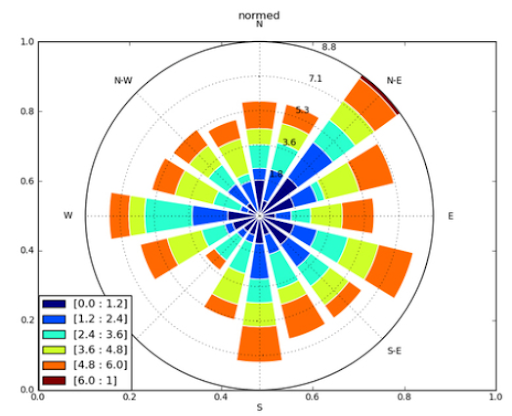
\includegraphics[width=\textwidth]{./images/Wind-rose}   
			\end{figure}	   
		\end{minipage}	
	\end{tabular}

		\scriptsize 
			특정 관측 지점에서 해당 기간동안 관측된 바람의 방향을 빈도와 함께 표기\\
			최근에는 풍향별 풍속계급 빈도도 그래프로 함께 나타냄

\end{frame}










\begin{frame}[t]{풍력 발전}
	\begin{tabular}{ll}
		\begin{minipage}[t]{0.45\textwidth}\scriptsize
			\begin{figure}[t]
				\includegraphics[trim=220 280 50 80, clip, page=209, width=0.9\textwidth]{\bookfile}
			\end{figure}	
				
			풍력 발전은 잠재적 가치가 높은 대체 에너지
		\end{minipage}	
		&
		\begin{minipage}[t]{0.5\textwidth} \scriptsize	
			\begin{figure}[t]
				\includegraphics[trim=100 550 270 50, clip, page=210, width=0.8\textwidth]{\bookfile}
			\end{figure}
			\questionset{풍력발전과 연관된 잠재적 환경문제는 무엇인가?}
			\solutionset{가장 큰 문제는 발전기 날개에 의해 새들이 죽는 것이다.\\
			또한 건설 과정에서 토지의 침식과 자연을 훼손하고, 미관을 해치기도 한다. \\
			또한 날개 회전시 발생하는 저주파도 큰 문제가 된다. }
		\end{minipage}
	\end{tabular}
\end{frame}


\begin{frame}[t]{풍력 발전}
	\begin{tabular}{ll}
		\begin{minipage}[t]{0.9\textwidth}\scriptsize
			\begin{figure}[t]
				\includegraphics[trim=125 230 260 350, clip, page=210, width=\textwidth]{\bookfile}
			\end{figure}
		\end{minipage}	
		&
		\begin{minipage}[t]{0.05\textwidth} \scriptsize	
		
		\end{minipage}
	\end{tabular}
\end{frame}



\section{추가 내용}




\begin{frame}[t]{기압경도력(PGF)}
	\begin{tabular}{ll}
		\begin{minipage}[t]{0.45\textwidth}\scriptsize
			\begin{figure}[t]
				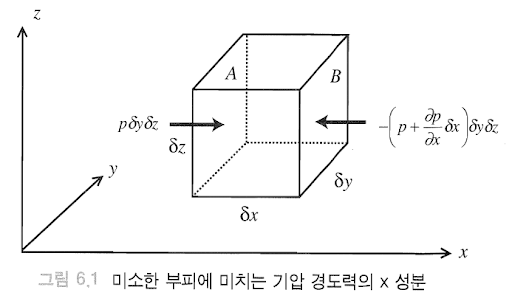
\includegraphics[width=\textwidth]{./images/PGF1}
			\end{figure}
			
		\end{minipage}	
		&
		\begin{minipage}[t]{0.5\textwidth} \scriptsize	
		압력은 단위 면적에 수직으로 작용하는 힘으로 정의되므로 정육면체 공기덩이에 작용하는 힘은 기압과 힘을 받는 면의 넓이의 곱으로 표현할 수 있다. 
			$${\displaystyle	{
					\begin{aligned}
						F_{x}&=p \delta y \delta z-\left(p+\frac{\partial p}{\partial x} \delta x\right) \delta y \delta z\\
						&=-\frac{\partial p}{\partial x} \delta x \delta y \delta z
					\end{aligned}
			}	} $$
		
				$m = \rho \delta x \delta y \delta z $ 이므로 단위 질량당 받는 힘은 각각

			$${\displaystyle	{
					\frac{F_{x}}{m} =-\frac{1}{\rho} \frac{\partial p}{\partial x}, \quad 
					\frac{F_{y}}{m} =-\frac{1}{\rho} \frac{\partial p}{\partial y}, \quad 
					\frac{F_{z}}{m} =-\frac{1}{\rho} \frac{\partial p}{\partial z} 
			}	}	$$

			$x$, $y$,  $z$ 각 성분별로 단위 벡터 $\boldsymbol{\hat{i}}$,  $\boldsymbol{\hat{j}}$, $\boldsymbol{\hat{k}}$	로 기압경도력을 표현하면

		\end{minipage}
	\end{tabular}
\end{frame}



\begin{frame}[t]{기압경도력(PGF)}
	\begin{tabular}{ll}
		\begin{minipage}[t]{0.45\textwidth}\scriptsize
			\begin{figure}[t]
				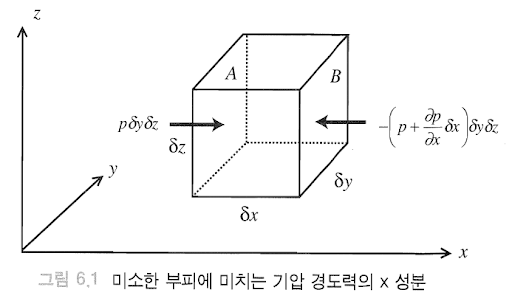
\includegraphics[width=\textwidth]{./images/PGF1}
			\end{figure}         
			
		\end{minipage}	                  
		&
		\begin{minipage}[t]{0.5\textwidth} \scriptsize	
			
			
			$${\displaystyle	{
					F_{PGF}=F_{x} \boldsymbol{\hat{i}}+{F}_{y} \boldsymbol{\hat{j}}+{F}_{z} \boldsymbol{\hat{k}}
			}	}	$$
			
			
			$${\displaystyle	{
					F_{PGF}=-\left(\frac{\partial p}{\partial x} \boldsymbol{\hat{i}}+\frac{\partial p}{\partial y} \boldsymbol{\hat{j}}+\frac{\partial p}{\partial z} \boldsymbol{\hat{k}}\right) \delta x \delta  y \delta  z
			}	}$$
			
			단위 질량당 기압경도력은 
			
			$${\displaystyle	{
					\nabla=\frac{\partial}{\partial x} \boldsymbol{\hat i}+\frac{\partial}{\partial y} \boldsymbol{\hat j}+\frac{\partial}{\partial z} \boldsymbol{\hat k}
			}	}$$
			
			$${\displaystyle	{
					\frac{F_{PGF}}{m}=-\frac{1}{\rho} \nabla p
			}	}$$
			
			\end{minipage}
		\end{tabular}
\end{frame}
	




\begin{frame}[t]{운동방정식}
	\begin{tabular}{ll}
		\begin{minipage}[t]{0.475\textwidth}\scriptsize

		대기의 운동에서 다루어지는 대부분의 현상에 사용되는 기본적인 운동방정식을 벡터로 표현한 것
		
		$${\displaystyle	{
				\frac{D\boldsymbol {\vec{U}}}{Dt} = -2 \Omega \times \boldsymbol {\vec{U}} - \frac{1}{\rho} \nabla p + \boldsymbol {\vec{g}} + \boldsymbol {\vec{F_r}}
		}	}	$$
		
		단, $ \boldsymbol {\vec{U}} = u \boldsymbol {\hat{i}} + v\boldsymbol {\hat{j}} + w\boldsymbol {\hat{k}}$ 로 3차원 속도 벡터이다.

		\end{minipage}	
		&
		\begin{minipage}[t]{0.475\textwidth} \scriptsize	
			\begin{figure}[t]
				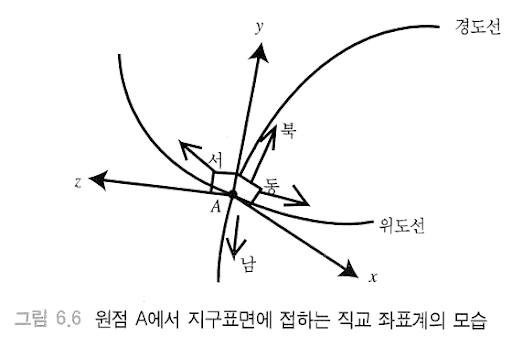
\includegraphics[width=\textwidth]{./images/xyz}
			\end{figure}

			회전좌표계에서의 운동방정식을 카테시안 좌표계에서 각 성분별로 나타내 보자.\\
			각각의 힘을 성분별로 나타내기 위해 지표 상의 원점 $\rm{A}$에 접한 평면 내에서 $x$축은 동쪽, $y$축은 북쪽, $z$축은 천정을 향하도록 정하자.\\
			
		\end{minipage}
	\end{tabular}
\end{frame}






\begin{frame}[t]{운동방정식}
	\begin{tabular}{ll}
		\begin{minipage}[t]{0.35\textwidth}\scriptsize
			\begin{figure}[t]
				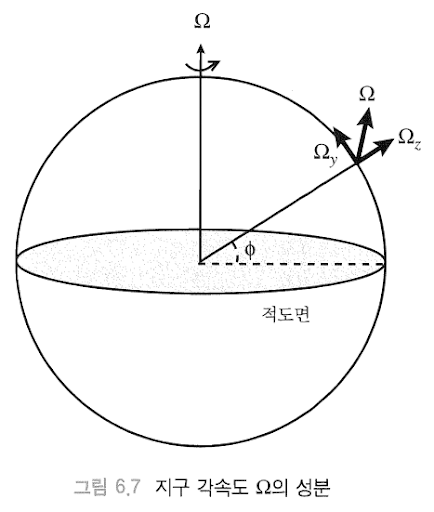
\includegraphics[width=\textwidth]{./images/coliolis}
			\end{figure}			
		\end{minipage}	
		&
		\begin{minipage}[t]{0.6\textwidth} \scriptsize	
			
				1) 전향력 : $-2 \Omega \times \boldsymbol {\vec{U}}$\\
		
				먼저 자전 각속도를 $\Omega$라고 할때 이를 각각 $x$, $y$, $z$ 성분으로 나누면, \\
				$\Omega_{x}=0$, $\Omega_{y}=\Omega \cos \varphi$, $\Omega_{z}=\Omega \sin \varphi$이다. \\
				
				$\boldsymbol {\vec{U}} = u \boldsymbol {\hat{i}} + v\boldsymbol {\hat{j}} + w\boldsymbol {\hat{k}}$이므로\\
				$${\displaystyle	{
						\begin{aligned}
							-2 \vec{\Omega} \times \boldsymbol{\vec{U}}
							& =
							-2\left|\begin{array}{ccc}\boldsymbol {\hat{i}} & \boldsymbol {\hat{j}} & \boldsymbol {\hat{k}} \\ 0 & \Omega \cos \varphi & \Omega \sin \varphi \\ u & v & w\end{array}\right|\\
							& =-2(\Omega w \cos \varphi-\Omega v \sin \varphi) \boldsymbol {\hat{i}}-2 \Omega u \sin \varphi \boldsymbol {\hat{j}}+2 \Omega u \cos \varphi \boldsymbol {\hat{k}}
						\end{aligned}
				}	}$$
				

		\end{minipage}
	\end{tabular}
\end{frame}





\begin{frame}[t]{운동방정식}
	\begin{tabular}{ll}
		\begin{minipage}[t]{0.475\textwidth}\scriptsize
			
			1) 전향력 : $-2 \Omega \times \boldsymbol {\vec{U}}$\\
			
			먼저 자전 각속도를 $\Omega$라고 할때 이를 각각 $x$, $y$, $z$ 성분으로 나누면, \\
			$\Omega_{x}=0$, $\Omega_{y}=\Omega \cos \varphi$, $\Omega_{z}=\Omega \sin \varphi$이다. \\
			
			$\boldsymbol {\vec{U}} = u \boldsymbol {\hat{i}} + v\boldsymbol {\hat{j}} + w\boldsymbol {\hat{k}}$이므로\\
			$${\displaystyle	{
					\begin{aligned}
						-2 \vec{\Omega} \times \boldsymbol{\vec{U}}
						& =
						-2\left|\begin{array}{ccc}\boldsymbol {\hat{i}} & \boldsymbol {\hat{j}} & \boldsymbol {\hat{k}} \\ 0 & \Omega \cos \varphi & \Omega \sin \varphi \\ u & v & w\end{array}\right|\\
						& =-2(\Omega w \cos \varphi-\Omega v \sin \varphi) \boldsymbol {\hat{i}}\\
						&~~~-2 \Omega u \sin \varphi \boldsymbol {\hat{j}}+2 \Omega u \cos \varphi \boldsymbol {\hat{k}}
					\end{aligned}
			}	}$$
			
			
		\end{minipage}	
		&
		\begin{minipage}[t]{0.475\textwidth} \scriptsize	
			
			2) 기압경도력
			
			$${\displaystyle	{
					-\frac{1}{\rho}	\nabla p = -\frac{1}{\rho}\frac{\partial p}{\partial x} \boldsymbol{\hat i} + -\frac{1}{\rho}\frac{\partial p}{\partial y} \boldsymbol{\hat j} + -\frac{1}{\rho}\frac{\partial p}{\partial z} \boldsymbol{\hat k}
			}	}$$
			
			
			3) 중력  
			
			$${\displaystyle	{ 
					\vec{g}=-g \boldsymbol{\hat{k}}
			}	}$$
			
			4) 마찰력
			
			$${\displaystyle	{            
					\overrightarrow{F_{r}}= \boldsymbol{\hat {i}} F_{x}+\boldsymbol{\hat{j} }F_{y}+\boldsymbol{\hat{k}} F_{z}
			}	}$$
			
		\end{minipage}
	\end{tabular}
\end{frame}



\begin{frame}[t]{운동방정식}
	\begin{tabular}{ll}
		\begin{minipage}[t]{0.475\textwidth}\scriptsize
			$1) \sim 4)$의 경우를 대입하여 카테시안 좌표계의 각 성분으로 나누어 표현하면
			$${\displaystyle {
				\begin{aligned}
					\frac{D u}{D t}&=-\frac{1}{\rho} \frac{\partial p}{\partial x}-2(\Omega w \cos \varphi-\Omega v \sin \varphi)+F_{x}\\
					\frac{D v}{D t}&=-\frac{1}{\rho} \frac{\partial p}{\partial y}-2 \Omega u \sin \varphi+F_{y}\\
					\frac{D w}{D t}&=-\frac{1}{\rho} \frac{\partial p}{\partial z}- g +2 \Omega u \cos \varphi+F_{z}
				\end{aligned}
			} }$$
			
		\end{minipage}	
		&
		\begin{minipage}[t]{0.475\textwidth} \scriptsize	
			코리올리 인자 $f =  2\Omega  \sin \varphi $로 나타내고, 값이 작은 항을 무시하면 
			$${\displaystyle 	{
				\begin{aligned}
					\frac{D u}{D t}&=-\frac{1}{\rho} \frac{\partial p}{\partial x} + 2\Omega v \sin \varphi = -\frac{1}{\rho} \frac{\partial p}{\partial x} + fv\\	
					\frac{D v}{D t}&=-\frac{1}{\rho} \frac{\partial p}{\partial y}-2 \Omega u \sin \varphi = -\frac{1}{\rho} \frac{\partial p}{\partial y}-fu\\
					0 &=-\frac{1}{\rho} \frac{\partial p}{\partial z}- g 
				\end{aligned}	
			}}	$$
		
		\end{minipage}
	\end{tabular}
\end{frame}



    
 
\begin{frame}[t]{자연좌표계}
	\begin{tabular}{ll}
		\begin{minipage}[t]{0.35\textwidth}\scriptsize
			\begin{figure}[t]
				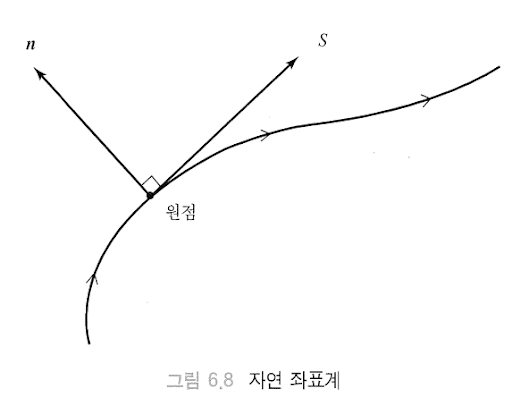
\includegraphics[width=\textwidth]{./images/SN}
			\end{figure}			
		\end{minipage}	
		&
		\begin{minipage}[t]{0.6\textwidth} \scriptsize
			대기운동은 매우 복잡하지만, 기압과 속도 분포는 다소 간단한 근사적인 힘의 균형에 의해 서로 연결되어 있다. \\
			수평적인 힘의 균형을 이해하기 위해 상황을 이상화 시켜 보자.\\
			- 마찰이 없음\\
			- 시간에 관계없이 일정한 공기 흐름 유지(시간에 독립적임)\\
			- 속도에 연직 성분 없음(수평 운동만 있다고 가정)\\
			자연좌표계는 $x$축(공기가 흐르는 방향)을 $s$축, $y$축(흐르는 방향의 왼쪽으로 수직한 방향)을 $n$축, 연직 방향을 $z$축으로 정의하고, \\
			자연좌표계 상에서 좌표($s$, $n$, $z$)의 방향을 
			각각 단위 벡터  $\boldsymbol{\hat{t}}$, $\boldsymbol{\hat{n}}$, $\boldsymbol{\hat{k}}$로 정의하면, 
			이런 체계에서 수평속도는 비음수 스칼라이며
			
			$${\displaystyle	{
					\vec{V}={V \boldsymbol{\hat{t}}}
			}	}$$
			따라서 운동을 따르면서 측정한 가속도는
			$${\displaystyle	{
				\frac{D \vec{V}}{D t}=\frac{D(V \boldsymbol{\hat{t}})}{D t}=\boldsymbol{\hat{t}} \frac{D V}{D t}+V \frac{D \boldsymbol{\hat{t}}}{D t}
			}	}$$
				
                    
		\end{minipage}
	\end{tabular}
\end{frame}
  
  
  
   
\begin{frame}[t]{자연좌표계}
 	\begin{tabular}{ll}
 		\begin{minipage}[t]{0.35\textwidth}\scriptsize
 			\begin{figure}[t]
 				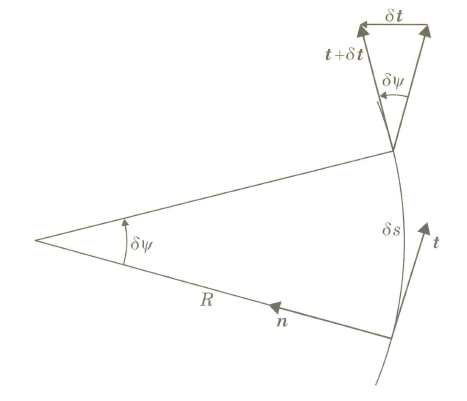
\includegraphics[width=\textwidth]{./images/SN1}
 			\end{figure}
 			$$ {\displaystyle {
 				\delta \psi=\frac{\delta s}{|R|}=\frac{|\delta \boldsymbol{\hat{t}}|}{|\boldsymbol{\hat{t}}|}
 				=|\delta \boldsymbol{\hat{t}}|
 			}}		$$
 			
 		\end{minipage}	
 		&
 		\begin{minipage}[t]{0.6\textwidth} \scriptsize
 			$\delta s \rightarrow 0$ 이 되도록 극한을 취하면 $\delta \boldsymbol{\hat t }$는 $\boldsymbol{\hat n }$과 평행한 방향이므로
 			
	 		$$	{\displaystyle{
					\begin{aligned}
	 					\frac{D \boldsymbol{\hat{t}}}{D s}&=\frac{\boldsymbol{\hat{n}}}{R}	\quad	\frac{D \boldsymbol{\hat{t}}}{D t}=\frac{D \boldsymbol{\hat{t}}}{D s}
			 				\frac{D s }{D t}	= \frac{\boldsymbol{\hat{n}}}{R}V\\
		 				\frac{D \vec{V}}{D t}&=\boldsymbol{\hat{t}} \frac{D V}{D t}+V \frac{D \boldsymbol{\hat{t}}}{D t}=\boldsymbol{\hat{t}} \frac{D V}{D t}+\boldsymbol {\hat{n}} \frac{V^{2}}{R}
					\end{aligned}
	 		}}$$

	 			전향력은 운동방향에 대해 연직으로 작용하므로 $-f \boldsymbol  {\hat{k}} \times \vec{V}=-f V \boldsymbol {\hat{n}}$\\
	 			기압경도력을 두 방향으로 분해하면, $-\frac{1}{\rho}\left(\frac{\partial p}{\partial s} \boldsymbol {\hat{t}}+\frac{\partial p}{\partial n} \boldsymbol {\hat{n}}\right) $ 이므로, 
	 			
	 			$${\displaystyle
	 				{
	 					\frac{D V}{D t} \boldsymbol {\hat{t}}+\frac{V^{2}}{R} \boldsymbol {\hat{n}}
	 					=-f V \boldsymbol {\hat{n}}-\frac{1}{\rho}\left(\frac{\partial p}{\partial s} \boldsymbol {\hat{t}}+\frac{\partial p}{\partial n} \boldsymbol {\hat{n}}\right)
	 			}}$$
 			각 성분별로 나타내면
	 			$${\displaystyle	{
	 					\frac{D V}{D t} 
	 					= -\frac{1}{\rho}\frac{\partial p}{\partial s}, 	\quad 	\frac{V^{2}}{R} + f V  = -\frac{1}{\rho}\frac{\partial p}{\partial n} 
	 			}}$$
 			
 		\end{minipage}
 	\end{tabular}
\end{frame}
    
%%
%
%
%
%
% 
% 
%관성풍
%$${\displaystyle {          
%	\frac{V^{2}}{R}+f  V = -\frac{1}{\rho}\frac{\partial p}{\partial s} 
%}}$$
%
%수평적으로 기압이 균일하여 기압경도력이 없는 경우에 발생하는 바람
%
%$${\displaystyle	{
%	\frac{\partial p}{\partial s} = 0, \quad 
%	\frac{\partial p}{\partial n} = 0
%}	}$$
%
%$${\displaystyle{
%	\frac{V^{2}}{R}+f  V = 0
%}	}$$
%
%곡률반지름  R에 대해서 풀면
%
%$${\displaystyle	{
%	{R} = -\frac{V}{f}, \quad  V = -fR
%}	}$$
%
%위도에 따른 f의 변화를 무시하면, 속력은 일정해야 하므로
%곡률 반지름도 일정
%북반구에서는 시계방향(고기압성 방향)으로 원을 그리는데
%이를 ‘관성원’이라고 부름
%
%        
%
%선형풍(Cyclostrophic wind)
%
%$${\displaystyle	{
%	\frac{V^{2}}{R}+f  V = -\frac{1}{\rho}\frac{\partial p}{\partial s} 
%}	}$$
%소규모 운동계에서는 곡률 반지름이 매우 작아서, 전향력보다 원심력이
%훨씬 커서 전향력을 무시할 수 있다. 
%원심력과 기압 경도력이 평형을 유지하며 등압선에 평행하게 부는 바람
%
%$${\displaystyle	{
%	\begin{aligned}
%		\frac{V^{2}}{R} &= -\frac{1}{\rho}\frac{\partial p}{\partial s}, \quad
%		V^{2} = -\frac{{R}}{\rho}\frac{\partial p}{\partial s} \\
%	V &= \sqrt {-\frac{{R}}{\rho}\frac{\partial p}{\partial s}}
%	\end{aligned}
%}	}$$
%
%
%기압경도력은 곡률 중심을 향하는 방향, 원심력은 멀어져 가는 방향
%





\begin{frame}[t]{경도풍의 풍속}
	\begin{tabular}{ll}
		\begin{minipage}[t]{0.475\textwidth}\scriptsize
			경도풍은 지압경도력과 전향력의 차이가 구심력으로 작용하여 부는 바람으로 자연 좌표계를 이용하여 표현하면, 
				$${\displaystyle	{
					\frac{V^2}{R} =-\frac{1}{\rho} \frac{\partial p}{\partial	n}-f V\\		
			}}$$
			$V$에 관한 2차 방정식으로 정리하여 근의 공식으로 근을 구하면, 
				$${\displaystyle	{
					\begin{aligned}
						&V^{2}+f R V+\frac{R}{\rho} \frac{\partial p}{\partial n}=0 \\ 
						&V=-\frac{f R}{2} \pm\sqrt {\frac{f^{2} R^{2}}{4}-\frac{R}{\rho} \frac{\partial p}{\partial n}}		
					\end{aligned}
				}}$$
			자연좌표계에서 $V$는 음수가 나올수 없으며, 루트 안에는 항상 양수이어여 실근을 가지므로
		\end{minipage}	
		&
		\begin{minipage}[t]{0.475\textwidth} \scriptsize
			근을 분류하여 먼저 
			$${\displaystyle	{
					V=-\frac{f R}{2} +\sqrt {\frac{f^{2} R^{2}}{4}-\frac{R}{\rho} \frac{\partial p}{\partial n}}		
			}	}$$		
			(1)	$R>0$, $- \frac{\partial p}{\partial n} > 0$
				$${\displaystyle	{
					\sqrt {\frac{f^{2} R^{2}}{4}-\frac{R}{\rho} \frac{\partial p}{\partial n}} > \frac{f|R|}{2}
				}	}$$
				$V$ 는 항상 $0$ 보다 크므로 정상 저기압\\
			        
			(2) $R>0$, $- \frac{\partial p}{\partial n} < 0$
				$${\displaystyle	{
					0 < \sqrt {\frac{f^{2} R^{2}}{4}-\frac{R}{\rho} \frac{\partial p}{\partial n}} < \frac{f|R|}{2}
				}	}$$
				$V$ 는 항상 $0$ 보다 작으므로 물리적으로 의미 없다.
		\end{minipage}
	\end{tabular}
\end{frame}



\begin{frame}[t]{경도풍의 풍속}
	\begin{tabular}{ll}
		\begin{minipage}[t]{0.475\textwidth}\scriptsize
			(3) $R<0$, $- \frac{\partial p}{\partial n} > 0$
				$${\displaystyle	{
					0 < \sqrt {\frac{f^{2} R^{2}}{4}-\frac{R}{\rho} \frac{\partial p}{\partial n}} < \frac{f|R|}{2}
				}	}$$
				$V$는 항상 ${\frac{f|R|}{2}}$ 보다 크므로 이상한 고기압\\
				
			(4) $R<0$, $- \frac{\partial p}{\partial n} < 0$
				$${\displaystyle	{
						\sqrt {\frac{f^{2} R^{2}}{4}-\frac{R}{\rho} \frac{\partial p}{\partial n}} > \frac{f|R|}{2}
				}}$$
				$V$는 항상 ${\frac{f|R|}{2}}$ 보다 크므로 이상한 저기압\\
		\end{minipage}	
		&
		\begin{minipage}[t]{0.475\textwidth} \scriptsize
			이제 아래의 근에 대하여 살펴보자.
			$${\displaystyle	{
					V=-\frac{f R}{2} -\sqrt {\frac{f^{2} R^{2}}{4}-\frac{R}{\rho} \frac{\partial p}{\partial n}}		
			}	}$$		
			
			(5)	$R>0$, $- \frac{\partial p}{\partial n} > 0$
				$${\displaystyle	{
					\sqrt {\frac{f^{2} R^{2}}{4}-\frac{R}{\rho} \frac{\partial p}{\partial n}} > \frac{f|R|}{2}
				}}$$
				$V$ 는 ${-{f|R|}}$ 보다 작으므로 물리적으로 의미 없다.\\
				
			(6) $R>0$, $- \frac{\partial p}{\partial n} < 0$
				$${\displaystyle	{
					0 < \sqrt {\frac{f^{2} R^{2}}{4}-\frac{R}{\rho} \frac{\partial p}{\partial n}} < \frac{f|R|}{2}
				}	}$$
				$V$ 는  ${-\frac{f|R|}{2}}$  보다 작으므로 물리적으로 의미 없다.\\
		\end{minipage}
	\end{tabular}
\end{frame}





\begin{frame}[t]{경도풍의 풍속}
	\begin{tabular}{ll}
		\begin{minipage}[t]{0.475\textwidth}\scriptsize
			(7) $R<0$, $- \frac{\partial p}{\partial n} > 0$
				$${\displaystyle	{
					0 < \sqrt {\frac{f^{2} R^{2}}{4}-\frac{R}{\rho} \frac{\partial p}{\partial n}} < \frac{f|R|}{2}
				}	}$$
				$V$는 항상  $0$ 보다 크고  ${\frac{f|R|}{2}}$ 보다 작으므로 정상 고기압\\
				
			(8) $R<0$, $- \frac{\partial p}{\partial n} < 0$
				$${\displaystyle	{
					\sqrt {\frac{f^{2} R^{2}}{4}-\frac{R}{\rho} \frac{\partial p}{\partial n}} > \frac{f|R|}{2}
				}	}$$
				$V$는 항상 $0$보다 작으므로 물리적으로 의미 없다.\\

		\end{minipage}	
		&
		\begin{minipage}[t]{0.475\textwidth} \scriptsize

		\end{minipage}
	\end{tabular}
\end{frame}





%
%
%
%%연속방정식
%%
%%카테시안 좌표계에 고정된 작은 체적소 $ \delta x \delta  y \delta  z$ 를 고려하자.
%%측면 통한 질량 유입의 순 비율은 체적 속에 축적되는 비율과 같아야 한다. 
%%
%%먼저, x방향에 대한 순 유입율을 계산하면, 단위 면적의 좌측면(A면)을 통한 질량 유입 비율은
%%
%%$${\displaystyle	{
%%		\left[\rho u\right]  \delta y \delta z
%%}	}$$
%%
%%오른쪽  B면을 통하여 고정된 부피 밖으로 질량이 빠져나가는 율은
%%
%%$${\displaystyle	{
%%	-\left[\rho u + \frac{\partial}{\partial x}(\rho v)\right] \delta y \delta z
%%}	}$$
%%
%%따라서 순 질량 유입량은
%%
%%$${\displaystyle	{
%%	(\rho u) \delta y \delta z-\left[\rho u+\frac{\partial(\rho u)}{\partial x} \delta x\right] \delta y \delta z=-\frac{\partial}{\partial x}(\rho u) \delta x \delta y \delta z
%%}	}$$
%%
%%
%%$${\displaystyle	{
%%	(\rho u) \delta y \delta z-\left[\rho u+\frac{\partial(\rho u)}{\partial x} \delta x\right] \delta y \delta z=-\frac{\partial}{\partial x}(\rho u) \delta x \delta y \delta z
%%}	}$$
%%
%%또한 y와 z 방향에 대해서도 위에 기술한 것처럼 유사하게 얻어진다.
%%
%%
%%$${\displaystyle	{
%%		(\rho u) \delta y \delta z-\left[\rho u+\frac{\partial(\rho u)}{\partial x} \delta x\right] \delta y \delta z=-\frac{\partial}{\partial x}(\rho u) \delta x \delta y \delta z
%%}	}$$
%%
%%
%%단위 부피당 질량 유입은
%%
%%$${\displaystyle	{
%%	-\nabla \cdot(\rho \vec{U})
%%}	}$$
%%
%%
%%
%%이는 국지 밀도 변화와 같으므로 다음과 같은 연속 방정식을 얻게 된다. 
%%
%%$${\displaystyle	{
%%	\frac{\partial \rho }{\partial t} +\nabla \cdot(\rho \vec{U}) = 0
%%}	}$$
%%
%%
%%움직임을 따르면서 측정한 공기덩이의 밀도증가율은 속도수렴과 같다.  즉, 속도 수렴이 있으면 밀도가 증가함을 뜻한다. 
%%
%%$${\displaystyle	{
%%	\frac{1}{\rho} \frac{D \rho}{D t}+\nabla \cdot \vec{U}=0
%%}	}$$
%
%
%
%
%
%
%
%
